\section{Time-Dependent FIFO Cost Functions}\label{sec:fifo-costs}

Time-dependent cost functions that follow the First In First Out (FIFO) rule are very important for the algorithms introduced later.
We begin by defining the FIFO rule in a directed graph $(V, E)$.


\begin{definition}
    A time-dependent cost function $c: \R\rightarrow \R_{\geq0}^E$ \emph{follows the FIFO rule} if for all edges $e\in E$ the function $T_e: \theta\mapsto \theta + c_e(\theta)$ is monotone increasing.
    It \emph{follows the strong FIFO rule} if $T_e$ is strictly increasing for all $e\in E$.
    The function $T_e$ is called \emph{traversal time} of $e$.
\end{definition}

For the following we concentrate on a graph $(V,E)$ where all nodes can reach a specific sink node $t\in V$.
Moreover, let $c:\R\rightarrow \R_{\geq0}^E$ be a time-dependent cost function.

The traversal time $T_P$ of a path $P = e_1\,\cdots\,e_k$ is given by the concatenation of the edges' traversal times as $T_P \coloneqq T_{e_k} \circ \cdots \circ T_{e_1}$.
The set of all simple $v$-$t$-Paths is denoted as $\paths_{v,t}$.
The \emph{earliest arrival time} at $t$ when starting at time $\theta$ in $v$ is then given by $l_{v,t}(\theta)\coloneqq \min_{P\in\paths_{v,t}} T_P(\theta)$.
Paths that attain this minimum are called \emph{shortest $v$-$t$-Path at time $\theta$}.

We call an edge $e=vw\in E$ \emph{active at time $\theta$}, if the condition $l_{v,t}(\theta) = l_{w,t}(T_e(\theta))$ holds true.
The set of active edges at time $\theta$ is collected in $E(\theta)$.
\todo[inline]{
    Isn't it disturbing, that these edges might not lie on a \textbf{simple} shortest path?
}

\subsection{Properties of FIFO Cost Functions}

To make sure that we can ignore non-simple paths in the definition of shortest paths, we exploit the FIFO property of the cost functions:

\begin{proposition}\label{prop:removing-cycles-in-fifo-graphs}
    Given cost functions $c:\R\rightarrow\R_{\geq0}^E$ following the FIFO rule, we can remove a cycle in any $v$-$t$-path $P$ while not increasing the path's traversal time.

    More specifically, if $P=P_1\, C \, P_2$ is the concatenation of paths $P_1$, a cycle $C$ and another path $P_2$, then it holds that $
        T_P(\theta) \geq \left(
        T_{P_2} \circ T_{P_1} \right)(\theta)$ for all $\theta\in\R$.
\end{proposition}
\begin{proof}
The statement is a direct consequence of the monotonicity of $T_{P_2}$ and the fact that $T_C(\theta) \geq \theta$ holds for all $\theta\in\R$.
\end{proof}

\begin{proposition}
    Let $c:\R\rightarrow\R_{>0}^E$ be a cost function following the FIFO rule.
    The vector $(l_v)_{v\in V}$ of functions is the maximal solution of the following system of equations in the function-valued variables $(\tilde l_v: \R \rightarrow \R)_{v\in V}$:
    \[
        \tilde l_v(\theta) = \begin{cases}
            \theta, &\text{if $v = t$}, \\
            \min_{\substack{
                e=vw\in\outEdges{v}               
            }} \tilde{l}_w\left(
                T_e(\theta)
            \right), &\text{otherwise}.
        \end{cases}
    \]
\end{proposition}
\begin{proof}
    To see that $(l_v)_{v\in V}$ is a solution of the system, we note that for $v = t$ we have $l_v(\theta) = \theta$ for all $\theta\in\R$.
    For $v\neq t$ let $e=vw\in\outEdges{v}$.
    Let $P$ be a shortest $w$-$t$-path at time $T_{e}(\theta)$.
    Let $P'\coloneqq e\circ P$ be the concatenation of $e$ and $P$.

    If $P'$ contains a cycle, then it must have been introduced by $e$ and $v$ must be visited a second time in $P'$.
    Removing this cycle gives a simple $v$-$t$-path $Q$ with 
    \[
        l_{v}(\theta) \leq T_{Q}(\theta)\leq T_{P'}(\theta) = l_{w}(T_{e}(\theta))
    \]
    by Proposition~\ref{prop:removing-cycles-in-fifo-graphs}.
    If $P'$ does not contain a cycle, we follow analogously
    \[
        l_{v}(\theta) \leq T_{P'}(\theta) = l_{w}(T_{e}(\theta)).
    \]
    This shows that $l_v(\theta)$ is a lower bound on $\{ \tilde l_w(
        T_{e}(\theta)
    ) \mid e=vw\in\outEdges{v}  \}$.
    Let $P = e_1\, \cdots\, e_k$ be a shortest $v$-$t$-path at time $\theta$ and let $e_1=vw$ and $P' = e_2\,\cdots\,e_k$.
    Furthermore, let $Q$ be a shortest $w$-$t$-path at time $T_{e_1}(\theta)$.
    Assume $T_{P}(\theta) > l_{w}(T_{e_1}(\theta))$.
    This implies
    \[
        T_{P}(\theta) > 
        T_{Q}(T_{e_1}(\theta)),
    \]
    such that removing any cycles in the path $e_1\circ Q$ would yield a shorter path than $P$.

    We now have to show that $(l_v)_{v\in V}$ is the maximal solution.
    That means that for any other solution $(\tilde l_v)_{v\in V}$ of the system of equations
     $\tilde l_v(\theta) \leq l_v(\theta)$ holds for all $v\in V$ and $\theta\in\R$.
    Let $P = e_1 \,\cdots e_k$ be a shortest $v$-$t$-path at time $\theta$ and let $v_0 = v, v_k= t$ and $e_i = v_{i-1} v_i$ for $i=1,\dots,k$.
    Then by the system of equations we infer \[
        \tilde l_{v}(\theta) \leq \tilde l_{v_1}(T_{e_1}(\theta)) \leq \tilde l_{v_2}(T_{e_1\,e_2} (\theta)) \leq \cdots \leq \tilde l_t(T_P(\theta)) = T_P(\theta) \leq l_v(\theta).
    \]
\end{proof}

\subsection{Duality of Arrival and Departure Times}

Sometimes it is useful not to work on the earliest arrival time, but the latest possible departure time.
To enable this switch, we define a kind of inverse of a monotonically increasing function:

\newcommand{\IncCoercive}{\mathcal{F}}
\begin{definition}
    We define the function space 
    \[
        \IncCoercive \coloneqq \left\{ f:\R \rightarrow \R \mid \text{ $f$ is increasing and $ \lim_{\abs{x}\rightarrow\infty} \abs{f(x)} = \infty$} \right\}.
    \]
    The \emph{reversal of $f\in\IncCoercive$} is defined as 
    \[
        \minv{f}:\R \rightarrow \R,\ \theta\mapsto \sup \{ \xi\in\R \mid f(\xi) \leq \theta \}.
    \]
\end{definition}

We can interpret the reversal of $f$ in the following way:
If $f(\theta)$ is the earliest arrival time when departing at time $\theta$, then $\minv{f}(\theta)$ is the latest departure time for arriving before or at time $\theta$.

\begin{proposition}\label{prop:reversal-props}
    For $f,g\in \IncCoercive$ the following statements are true:
    \begin{enumerate}[label=(\roman*)]
        \item\label{prop:reversal-props:inner-operator} It holds that $\minv{f}\in\IncCoercive$, i.e. $\minv{f}$ is increasing and $\lim_{\abs{x}\rightarrow\infty} \abs{f(x)} = \infty$.
        \item\label{prop:reversal-props:continuous} If $f$ is continuous, then $\minv{f}(\theta) = \max \{ \xi\in\R \mid f(\xi) = \theta \}$ holds for all $\theta\in\R$ and $\minv{f}$ is strictly increasing.
        Moreover, we have $f\circ \minv{f} = \id_\R$.
        \item\label{prop:reversal-props:inverse} If $f$ is continuous and strictly increasing, then  $\minv{f}$ is the inverse of $f$.
        \item\label{prop:reversal-props:composition-minimum} It holds that $\minv{(g\circ f)} = \minv{f}\circ\minv{g}$ and $\minv{(\min\{f,g\})} = \max\{\minv{f}, \minv{g}\}$.
        \item\label{prop:reversal-props:flip-id} If $f\geq \id_\R$ holds pointwise, then so does $\minv{f} \leq \id_\R$.
    \end{enumerate}
\end{proposition}
\begin{proof}
    \ref{prop:reversal-props:inner-operator}. 
    Let $\theta_1, \theta_2\in\R$ with $\theta_1 < \theta_2$.
    Then \begin{equation}\label{eq:reversal-props:increasing}
        \minv{f}(\theta_1) = \sup\{\xi\in\R \mid f(\xi) \leq \theta_1 \}
        \leq \sup\{\xi\in\R \mid f(\xi)\leq \theta_2 \} = \minv{f}(\theta_2)
    \end{equation}
    implies the monotonicity.
    From $\lim_{\abs{\theta}\rightarrow \infty} \abs{f(\theta)}$ and the monotonicity of $f$ we conclude \[
        \lim_{\abs{\theta}\rightarrow \infty} \abs{\minv{f}(\theta)}
        = \lim_{\abs{\theta}\rightarrow \infty} \abs{ \sup\{\xi\in\R \mid f(\xi)\leq \theta \} } = \infty.
    \]

    \ref{prop:reversal-props:continuous}.
    We note, that $\{ \xi\in\R \mid f(\xi) = \theta \}$ is non-empty, closed and bounded from above because of the condition $\lim_{\abs{\theta}\rightarrow \infty} \abs{f(\theta)} = \infty$ and the continuity and monotonicity of $f$.
    The reversal $\minv{f}$ is strictly increasing as the inequality~\eqref{eq:reversal-props:increasing} is strict for continuous $f$.
    
    \ref{prop:reversal-props:inverse}.
    Let $f$ be continuous and strictly increasing.
    Then it holds that 
    \[
        \minv{f}(\theta) = \max\{\xi\mid f(\xi) = \theta \} = f^{-1}(\theta).
    \]

    \ref{prop:reversal-props:composition-minimum}.
    After inserting the definition the first statement evaluated in $\theta$ becomes
    \[
        l\coloneqq \sup\left\{
            \xi \mid g(f(\xi)) \leq \theta
        \right\}
        =
        \sup\left\{
            \xi_f \mid f(\xi_f) \leq
            \sup\left\{ \xi_g \mid g(\xi_g) \leq \theta \right\}
            \right\}
         \eqqcolon r.
    \]
    Let $\xi_f\in\R$ fulfill $f(\xi_f) \leq \minv{g}(\theta)$.
    Then for all $\xi_g$ with $g(\xi_g) \leq \theta$ we have $f(\xi_f) \leq \xi_g$.
    Then because of the monotonicity of $g$ and $f$ we follow $g(f(\xi_f)) \leq g(\xi_g) \leq \theta$ which implies $l \geq r$.
    To see that $r\geq l$ holds, any $\xi\in\R$ with $g(f(\xi)) \leq \theta$ fulfills $f(\xi)\leq \minv{g}(\theta)$.

    The statement on the minimum of $f$ and $g$ evaluated in $\theta$ is of the form
    \[
        l\coloneqq \sup\{\xi \mid \min\{f(\xi),g(\xi)\} \leq \theta \}
        =
        \max\{
            \sup\{\xi \mid f(\xi)\leq \theta \},
            \sup\{\xi\mid g(\xi)\leq\theta\}
        \} \eqqcolon r.
    \]
    Let $\xi\in\R$ fulfill $\min\{f(\xi),g(\xi)\}\leq \theta$ and assume $f(\xi)\leq g(\xi)$ without loss of generality.
    Then it holds that $f(\xi) \leq \theta$ and therefore $\xi \leq \minv{f}(\theta)\leq r$ implying $l\leq r$.
    On the contrary, assume $\minv{f}(\theta)\leq \minv{g}(\theta)$ without loss of generality, so that $r = \minv{g}(\theta)$.
    Any $\xi\in\R$ with $g(\xi)\leq \theta$ fulfills $\min\{f(\xi),g(\xi)\}\leq g(\xi)\leq\theta$ and hence $l \geq r$ holds true.

    \ref{prop:reversal-props:flip-id}.
    For $f\geq \id_R$ we deduce for all $\theta\in\R$ \[
        \minv{f}(\theta) = \sup\{ \xi\in\R \mid f(\xi) \leq \theta \}
        \leq \sup\{\xi\in\R \mid \xi \leq \theta \} = \theta. \qedhere
    \]
\end{proof}

\begin{corollary}
    For a cost-function $c:\R\rightarrow\R_{\geq0}^E$, that follows the FIFO rule and that fulfills $\lim_{\theta\to-\infty} T_e(\theta) = -\infty$, the following statements hold true:
    \begin{enumerate}[label=(\roman*)]
        \item For all edges $e\in E$ we have $T_e \in \IncCoercive$.
        \item\label{prop:reversal-props:paths} For any path $P=e_1\,\cdots \,e_k$ it holds that $\minv{T_P} = \minv{T_{e_1}} \circ \cdots \circ \minv{T_{e_k}}$.
        \item For any node $v\in V$ it holds that $\minv{l_{v,t}} = \max_{P\in\paths_{v,t}} \minv{T_P}$.
    \end{enumerate}
\end{corollary}

The reversal of a function can be utilized for a characterization of active edges:

\begin{lemma}\label{lem:characterization-active-edges}
    Let $c: \R\rightarrow\R_{\geq0}^E$ be a continuous cost function following the FIFO rule with $\lim_{\theta\to-\infty} T_e(\theta) = -\infty$ for all $e\in E$ and let $t\in V$ be a sink node.
    Then an edge $e=vw$ is active at time $\theta$ if and only if $T_e(\theta) \leq \minv{l_{w,t}}( l_{v,t}(\theta) )$.
\end{lemma}
\begin{proof}
    The edge $e$ is by definition active at time $\theta$ if and only if 
    Let edge $e$ be active at time $\theta$ which means $l_{w,t}(T_e(\theta)) \leq l_{v,t}(\theta)$.
    By definition of the reversal this already implies $\minv{l_{w,t}}(l_{v,t}(\theta)) \geq T_e(\theta)$.

    If on the contrary $T_e(\theta) \leq \minv{l_{w,t}}( l_{v,t}(\theta) )$ holds, then the monotonicity of $l_{w,t}$ implies 
    \[
        l_{w,t}( T_e(\theta) ) \leq l_{w,t}\left(\minv{l_{w,t}}(l_{v,t}(\theta))\right),
    \]
    and by the continuity of $l_{w,t}$ the claim follows because Proposition~\ref{prop:reversal-props}~\ref{prop:reversal-props:continuous} states that $l_{w,t} \circ \minv{l_{w,t}} = \id_\R$. 
\end{proof}

\subsection{The Dynamic Dijkstra Algorithm}

The first algorithm we discuss is a simple modification of the Dijkstra Algorithm to determine the earliest arrival times $(l_{s,w}(\theta))_{w\in V'}$ at nodes of some subset $V'\subseteq V$ when departing from a source node $s$ at time $\theta$.
Here, only those nodes are relevant for us that are reachable from $s$ and that can reach $t$.
Moreover, we only need to determine the arrival times of nodes $w$ that can be reached before $t$, i.e. that fulfill $l_{s,w}(\theta) \leq l_{s,t}(\theta)$.
Hence, the set $V'$ consists of all nodes $w$ that lie on a path from $v$ to $t$ and fulfill $l_{s,w}(\theta) \leq l_{s,t}(\theta)$.

\begin{algorithm}[ht]
\begin{minted}[mathescape, linenos]{python}
def dynamic_dijkstra(
    theta: float, source: Node, sink: Node, relevant_nodes: Set[Node],
    costs: List[Callable[[float], float]]
) -> Dict[Node, float]:
  arrival_times: Dict[Node, float] = {}
  queue: PriorityQueue[Node] = PriorityQueue([(source, theta)])
  while len(queue) > 0:
    arrival_time, v = queue.min_key(), queue.pop()
    arrival_times[v] = arrival_time
    if v == sink:
      break
    for e in v.outgoing_edges:
      w = e.node_to
      if w in arrival_times.keys() or w not in relevant_nodes:
        continue
      relaxation = arrival_time + costs[e.id](arrival_time)
      if not queue.contains(w):
        queue.push(w, relaxation)
      elif relaxation < queue.key_of(w):
        queue.decrease_key(w, relaxation)
  return arrival_times
\end{minted}
\caption{The Dynamic Dijkstra Algorithm}
\label{alg:dynamic-dijkstra}
\end{algorithm}

Adjusting the classical Dijkstra Algorithm for static edge costs to our setting yields the Dynamic Dijkstra Algorithm as depicted in Algorithm~\ref{alg:dynamic-dijkstra}.

A priority queue, consisting of items together with a priority key associated with each item, operates at the heart of the algorithm.
This queue has to support the operations \code{push(item, key)}, \code{min_key()}, \code{pop()}, \code{decrease_key(item, new_key)} as well as \code{contains(item)}.
The operation \code{push(item, key)} adds the item \code{item} with priority \code{key} to the queue, \code{min_key()} returns the minimum key of an item in the queue, \code{pop()} returns the item with minimum key and removes it from the queue, \code{contains(item)} returns whether \code{item} is contained in the queue and the operation \code{decrease_key(item, new_key)} replaces the priority key associated to the item \code{item} with \code{new_key}.


The idea of Algorithm~\ref{alg:dynamic-dijkstra} is to iteratively retrieve an unvisited node $v$ with the current earliest arrival time $t$ of all unvisited nodes.
Then, for each outgoing edge $e=vw$ we realize its cost at time $t$ and update the arrival time of the target node $w$.
The priority queue holds all discovered but unvisited nodes where the priority key of a node $w$ is its currently suspected earliest arrival time, an upper bound on $l_{s,w}(\theta)$.
Nodes that are not added to the queue have either been already visited and thus have an entry in \code{arrival_times} or are not discovered and hence have an imaginary arrival time of $\infty$.

In the following proposition we show the correctness of the algorithm:

\begin{proposition}
    Given cost functions $c:\R \rightarrow \R_{\geq0}^E$ following the FIFO rule, the Dynamic Dijkstra Algorithm initiated on the source $s\in V$ and a reachable sink $t\in V$ computes the vector $(l_{s,w}(\theta))_{w\in V'}$ with \[
        V' = \{ w\in V \mid \text{$w$ lies on an $s$-$t$-path and $l_{s,w}(\theta) \leq l_{s,t}(\theta)$} \}.
    \]
\end{proposition}
\begin{proof}
    As an invariant for the algorithm we proof, that once a value of a node $w$ is written to \code{arrival_times[w]}, this value coincides with $l_{s,w}(\theta)$.
    In the beginning this is clearly true as \code{arrival_times} is initially empty.
    In the first iteration of the loop, the variable $\code{v}$ holds the source $s$ and its key $\theta= l_{s,s}(\theta)$ is written to \code{arrival_times[v]}.
    Assume the loop invariant holds before entering the body of the loop again at a later time and let $v$ be the popped node.
    As nodes are added at most once to the queue, we have $v \neq s$.
    Let $u$ be the node in whose iteration $v$ was added to the queue or the key of $v$ in the queue was decreased the most recently.
    The invariant implies $\code{arrival_times[}u\code{]} = l_{v,u}(\theta)$ and thus $\code{arrival_time} = l_{s,u}(\theta) + c_{uv}(l_{s,u}(\theta)) = T_{uv}(l_{s,u}(\theta)) \geq l_{s,v}(\theta)$.

    Assume $\code{arrival_time} > l_{s,v}(\theta)$ and let $P$ be a shortest $s$-$v$-path at time $\theta$.
    If all nodes of $P$ were available in \code{arrival_times}, then the last node before $v$ in $P$ would have set the key of $v$ in its iteration to $l_{s,v}(\theta)$.
    Let $u$ be the first node in $P$ that is not available in \code{arrival_times}.
    Because $u$ cannot be the source $s$, the  predecessor $u'$ of $u$ in $P$ must have set the key of $u$ to at most $T_{u'u}(l_{s,u'}(\theta)) \leq T_P(\theta)$.
    As $\code{arrival_time}>l_{s,v}(\theta) = l_P(\theta)$ the key of $u$ in the queue was smaller than the key of $v$, so the priority queue would have popped $u$ before $v$.
\end{proof}

A simple binary min-heap together with a lookup table was implemented to support the operations of the queue efficiently.
With this data structure, the worst case running time is logarithmic in the number of queue items for the operations \code{push(item, key)}, \code{pop()} and \code{decrease_key(item, new_key)} and constant for the operations \code{min_key()} and \code{contains(item)}.
Thus, the Dynamic Dijkstra Algorithm terminates with a running time of $\bigO( (\abs{V} + \abs{E}) \cdot \log \abs{V})$.


\subsection{Computing Active Outgoing Edges}\label{sec:compute-active-edges}

Given a FIFO cost function $c: \R\rightarrow\R_{\geq0}^E$ with nodes $s,t\in V$, a time $\theta\in\R$, we want to compute the active outgoing edges $E(\theta) \cap \outEdges{s}$ of $s$, i.e. the edges $e=sw$ with 
\[
    l_{s,t}(\theta) = l_{w,t}(T_e(\theta)).
\]
Unfortunately, from the arrival times $(l_{s,w}(\theta))_{w\in V'}$ obtained by a simple run of the Dynamic Dijkstra Algorithm, we cannot determine all active edges:
Usually, the idea is to backtrack all shortest paths by searching edges $e=vw$ backwards starting from $t$ for which equality holds in $l_{s,w}(\theta) \leq T_e(l_{s,v}(\theta))$.
This approach is described in Algorithm~\ref{alg:backward-search} which aims to return the set $E(\theta)\cap \outEdges{s}$.
The vector $(l_{s,w}(\theta))_{w\in V'}$ as returned by the Dynamic Dijkstra Algorithm is passed to the function via the parameter \code{arrivals}.
During the procedure, we only enqueue a node $u$ to the queue \code{queue}, if there exists a path from $u$ to $t$ in which each edge $e=vw$ fulfills $l_{s,w}(\theta)= T_e(l_{s,v}(\theta))$.
Once we discover an edge from $s$ to such an enqueued node that also fulfills the equality, we add it to the set of active outgoing edges of $s$ which is returned by the algorithm.

\begin{algorithm}
    \begin{minted}[mathescape, linenos]{python}
def backtrack_shortest_paths(
  costs: List[Callable[[float], float]], arrivals: Dict[Node, float],
  source: Node, sink: Node
) -> Set[Edge]:
  active_edges = set()
  queue: List[Node] = [sink]
  discovered: Set[Node] = {sink}
  while len(queue) > 0:
    w = queue.pop()
    for e in w.incoming_edges:
      v = e.node_from
      if v not in arrivals.keys():
        continue
      if arrivals[v] + costs[e.id](arrivals[v]) <= arrivals[w]:
        if v == source:
          active_edges.add(e)
        if v not in discovered:
          queue.append(v)
          discovered.add(v)
  return active_edges
    \end{minted}
    \caption{Retrieve Active Edges by Backtracking Shortest Paths}
    \label{alg:backward-search}
\end{algorithm}

The following proposition proves that paths found using the described approach are in fact shortest paths.
Moreover, we show that for strong FIFO costs we find all shortest paths.
That means, for strong FIFO costs, Algorithm~\ref{alg:backward-search} returns the whole set $E(\theta)\cap\outEdges{s}$.

\begin{proposition}
    Let $P=e_1\,\cdots\,e_k$ be a path with $e_i = v_{i-1}v_{i}$ and $v_0 = s, v_k= t$ and let $c:\R\rightarrow\R^E_{\geq0}$ be a cost function following the FIFO rule. Then
    \[ 
        \left(\forall i:\, {T_{e_i}}{\left(l_{s,v_{i-1}}(\theta)\right)} = l_{s,v_i}(\theta)\right)
        \implies
        T_P(\theta) = l_{s,t}(\theta).
    \]
    If $c$ follows the strong FIFO rule, the statements are equivalent.
\end{proposition}

\begin{proof}
    Assume $T_{e_i}(l_{s,v_{i-1}}(\theta)) = l_{s,v_i}(\theta)$ holds for all $i$.
    Then we have \begin{align*}
        T_P(\theta)
        &= T_P(l_{s,s}(\theta))
        = T_{e_2\,\cdots\,e_{k-1}}(l_{s,v_1}(\theta))
        = \cdots
        = l_{s,v_k}(\theta) = l_{s,t}(\theta).
    \end{align*}

    Let $c$ now follow the strong FIFO rule and assume there is some $i\in\{1,\dots, k\}$ with $T_{e_i}(l_{s,v_{i-1}}(\theta)) > l_{s,v_i}(\theta)$.
    Let $P'$ be a shortest $s$-$v_i$-path at time $\theta$.
    If we extend $P'$ with $e_{i+1}\,\cdots\,e_{k}$ we get an $s$-$t$-path $P''$ which 
    by the strong monotonicity of all $T_e$ fulfills \[
        l_{s,t}(\theta) \leq T_{P''}(\theta)
        = T_{e_{i+1}\,\cdots\,e_k}(l_{s,v_{i}}(\theta))
        < T_{e_{i+1}\,\cdots\,e_k}(T_{e_1\,\cdots\,e_i}(\theta))
        = T_P(\theta).\qedhere
    \]
\end{proof}

For general FIFO costs however, not all subpaths of shortest paths are again shortest paths.
That means, there might be edges $e=vw$ that do not fulfill the equality $l_{s,w}(\theta) = T_e(l_{s,v}(\theta))$ but still lie on a shortest $s$-$t$-path at time $\theta$.
This might be the case if a bottleneck edge $e'$ closer to $t$ has an interval on which $T_{e'}$ is constant.
An example of this can be seen in Figure~\ref{fig:bottleneck}.

\begin{figure}
    \centering
    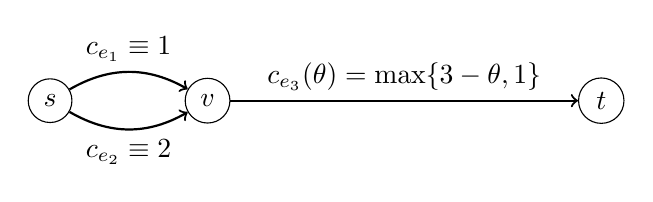
\begin{tikzpicture}
        \node[draw,circle](0)at(0,1) {$s$};
        \node[draw,circle](1)at(2, 1) {$v$};
        \node[draw,circle](2)at(7,1) {$t$};
        
        \draw[thick,->, bend left](0) to[bend left] node[above]{$c_{e_1}\equiv 1$} (1);
        \draw[thick,->](0) to[bend right] node[below]{$c_{e_2}\equiv 2$} (1);
        \draw[thick,->](1) --node[above]{$c_{e_3}(\theta) = \max\{ 3 - \theta, 1\}$} (2);
    \end{tikzpicture}
    \caption{Both $e_1$ and $e_2$ are active at time $0$ with $T_{e_2}(l_{s,s}(0))> l_{s,v}(0)$.}\label{fig:bottleneck}
\end{figure}

This leaves us with the question of how to find the rest of the active edges for general FIFO cost functions.
For the rest of this section, let $c:\R\rightarrow\R^E_{\geq0}$ be a continuous cost function following the FIFO rule with $\lim_{\theta\to-\infty} T_e(\theta) = -\infty$ for all $e\in E$.
Now we want to exploit that once we determined $l_{s,t}(\theta)$, we can do another run of the Dynamic Dijkstra Algorithm on the reverse graph $\rev{G} = (V, \rev{E})$ with $\rev{E}\coloneqq \{ \rev{e} = wv \mid e=vw\in E \}$ to compute the latest departure time starting from any node $v$ to arrive before or at time $l_{s,t}(\theta)$ at $t$.

We define the corresponding cost function $\tilde c$ as \[
    \tilde c : \R \rightarrow \R_{\geq0}^{\rev E}, \quad
    \tilde c_{\rev e}(\theta) \coloneqq - \minv{T_e}(-\theta) - \theta.
\]
Note, that $T_e  \geq \id_\R$ and by Proposition~\ref{prop:reversal-props}~\ref{prop:reversal-props:flip-id} we infer $\minv{T_e} \leq \id_\R$.
Therefore, we have $\minv{T_e}(-\theta) \leq -\theta$ and thus $\tilde c_{\rev e}(\theta) \geq 0$.

We denote the traversal times induced by $\tilde c$ by $\tilde T_{\rev e}$ and $\tilde T_{\rev P}$,where $\rev P = \rev{e_k} \, \cdots \, \rev{e_1}$ for $P = e_1\,\cdots\, e_k$,
and the earliest arrival time due to $\tilde c$ as $\tilde l_{v,w}$.
The traversal times fulfill $\tilde T_e = -\minv{T_e}(-\theta)$ which is by Proposition~\ref{prop:reversal-props}~\ref{prop:reversal-props:continuous} strictly increasing.
Hence, $\tilde c$ follows the strong FIFO rule.
For a path $\rev{P} = \rev{e_k}\,\cdots\, \rev{e_1}$ the traversal time yields
\[
    \tilde T_{\rev P} (\theta)
    = \tilde T_{\rev{e_{k-1}}\,\cdots\,\rev{e_1}}(- \minv{T_{e_k}} ( - \theta ))
    = \tilde T_{\rev{e_{k-2}}\,\cdots\,\rev{e_1}}(-\minv{T_{e_{k-1}}} (\minv{T_{e_k}} ( - \theta ))
    = \cdots
    = - \minv{T_P}(-\theta)
\]
and the earliest arrival times are of the form
\[
    \tilde l_{v,w}(\theta)
    = \min_{P\in\paths_{w,v}} \tilde T_{\rev{P}}(\theta)
    = \min_{P\in\paths_{w,v}} - \minv{T_P}(-\theta)
    = - \max_{P\in\paths_{w,v}} \minv{T_P}(-\theta)
    = - \minv{l_{w,v}}(-\theta)
\]

With this setup, we can do a second run of the Dynamic Dijkstra Algorithm to obtain the vector \[
    (\tilde l_{t,w}( - l_{s,t}(\theta) ))_w = (- \minv{l_{t,w}}( l_{s,t}(\theta) ))_w.
\]
Using Lemma~\ref{lem:characterization-active-edges} we can now check whether an outgoing edge $sw\in\outEdges{s}$ of $s$ is active at time $\theta$ by evaluating $T_e(\theta) \leq \minv{l_{t,w}}( l_{s,t}(\theta))$.

\begin{algorithm}[ht]
    \begin{minted}[mathescape, linenos]{python}
def get_active_edges(
  costs: List[PiecewiseLinear], theta: float, source: Node, sink: Node,
  relevant_nodes: Set[Node], graph: DirectedGraph, strong_fifo: bool
) -> Set[Edge]:
  if len(source.outgoing_edges) <= 1:
    return source.outgoing_edges
  arrivals = dynamic_dijkstra(
    theta, source, sink, relevant_nodes, costs
  )
  if strong_fifo:
    return backtrack_shortest_paths(costs, arrivals, source, sink)
  else: # Second run of Dijkstra on the reverse graph.
    graph.reverse()
    traversals = [cost + identity for cost in costs]
    new_costs: List[Callable[[float], float]] = [
      lambda t: -trav.reversal(-t) - t for trav in traversals
    ]
    neg_departures = dynamic_dijkstra(
      -arrivals[sink], sink, source, relevant_nodes, new_costs
    )
    graph.reverse()
    return [
      e for e in source.outgoing_edges
      if traversals[e.id](theta) <= -neg_departures[e.node_to]
    ]
  \end{minted}
  \caption{Calculating Active Edges}
  \label{alg:calculate-active-edges}
\end{algorithm}


To implement this algorithm, we have to restrict ourselves to cost functions where the reversal of $T_e$ can be evaluated easily.
This is the case, for example, if $c_e$ are piecewise linear functions.
The resulting algorithm for this class of functions can be seen in Algorithm~\ref{alg:calculate-active-edges}.
Here, the flag \code{strong_fifo} is expected to be set only for cost functions following the strong FIFO rule.
For these type of functions, we use the simpler backtracking search; for  general FIFO functions, we use the approach described above.
Other than that, if $s$ has only up to one outgoing edge, we simply return $\outEdges{s}$.


\subsection{Computing the Arrival Functions}

Often, it is useful not only to compute active edges at some fixed point in time, but to have the earliest arrival functions $(l_{v,t})_{v\in V'}$ at some sink available as functions over time.

A very simple but also quite expensive method of computing these functions is a modification of the Bellman-Ford algorithm. \todo{Add cite}
It uses the representation found in Proposition~\ref{prop:characterization-arrival-functions}.
This means, we want to find the maximal solution of the system of equations \[
    \tilde l_v(\theta) = \begin{cases}
        \theta, &\text{if $v = t$}, \\
        \min_{\substack{
            e=vw\in\outEdges{v}               
        }} \tilde{l}_w\left(
            T_e(\theta)
        \right), &\text{otherwise}.
    \end{cases}
\]
Hence, the idea is to initialize all functions with $\tilde l_v(\theta) \coloneqq \infty$ for $v\neq t$ and $\tilde l_t(\theta) \coloneqq \theta$ and decrease the functions (pointwise) using the operation $\tilde l_v \coloneqq \min_{vw\in\outEdges{v}} \tilde l_w \circ T_{vw}$ until no further changes are made, and the equations are fulfilled for all $v\in V$.

More specifically, if some function $\tilde l_w$ changes, then all nodes $v$ with an edge $vw$ leading to $w$ might need to be adjusted as well using the operation $\tilde l_v \coloneqq \min\{ \tilde l_v, \tilde l_w \circ T_{vw} \}$.
Therefore, we need some operations on the class of functions operated on to formulate the algorithm:
To calculate the traversal times $T_e = c_e + \id_\R$ we need pointwise addition and a representation of the identity function; for updates of the functions the pointwise minimum and the composition of functions have to be implemented.
To detect changes we also need to be able to identify whether one function is everywhere smaller or equal to some other function. 
Instead of representing the constant function with value $\infty$, we can simply only add a function once it gets its first update.

\begin{algorithm}[h]
    \begin{minted}[mathescape,
        linenos,
        numbersep=5pt,
        framesep=5mm]{python}
def dynamic_bellman_ford(
    sink: Node, costs: List[PiecewiseLinear], relevant_nodes: Set[Node],
    theta: float
) -> Dict[Node, PiecewiseLinear]:
    arrivals: Dict[Node, PiecewiseLinear] = { sink: identity }
    traversals = [cost + identity for cost in costs]
    changed_nodes = {sink}
    while len(changed_nodes) > 0:
        change_detected = {}
        for w in changed_nodes:
            for e in w.incoming_edges:
                v = e.node_from
                if v not in relevant_nodes:
                    continue
                relaxation = arrivals[w].compose(traversals[e.id])
                if v not in arrivals.keys():
                    change_detected.add(v)
                    arrivals[v] = relaxation
                elif not arrivals[v] <= relaxation:
                    change_detected.add(v)
                    arrivals[v] = arrivals[v].minimum(relaxation)
        changed_nodes = change_detected
    return arrivals
    \end{minted}
    \caption{Dynamic Bellman-Ford Algorithm}
    \label{alg:dynamic-bellman-ford}
\end{algorithm}

All the necessary operations explained above have been created for piecewise linear functions.
The resulting procedure is shown in Algorithm~\ref{alg:dynamic-bellman-ford}.
Here, \code{cost + identity} is the piecewise linear function representing the sum of \code{cost} and \code{identity}, the expression \code{arrivals[w].compose(traversals[e.id])} computes the piecewise linear function representing $\code{arrivals[w]}\circ \code{traversals[e.id]}$.
The decision whether the inequality $\code{arrivals[v]}(\theta) \leq \code{relaxation}(\theta)$ holds for all $\theta \in \R$ is expressed by the term \code{arrivals[v] <= relaxation}. 
Finally, the pointwise minimum of the functions \code{arrivals[v]} and \code{relaxation} is computed by \code{arrivals[v].minimum(relaxation)}.


The benefit of calculating the arrival times as functions is that the active outgoing edges of all nodes $v$ can be determined in one run of the Dynamic Bellman-Ford Algorithm by simply evaluating $l_{w,t}(T_e(\theta)) \leq  l_{v,t}(\theta)$ for $vw\in E$.